% TeX root=../main.tex
\section{Sistema de escrita}

\lipsum[4]

\section{Fonologia}

\lipsum[3]

\section{Flexão nominal}

\lipsum[1]

\section{Leitura: BABYLON 3}

Trata-se de um vaso em estado fragmentário (quatro pedaços) escavado por
Koldewey na década de 20 onde se acredita ser a cidade de Babilônia, sítio
arqueológico de Arpada, noroeste de Aleppo (Síria), contendo uma inscrição no
beiral em cursivas de baixo relevo, sentido sinistroverso, em duas linhas a
serem lidas em conjunto (para cada coluna, lê-se o caractere na primeira linha,
em seguida o da segunda linha e assim sucessivamente).

\begin{figure}[ht!]
	\begin{center}
		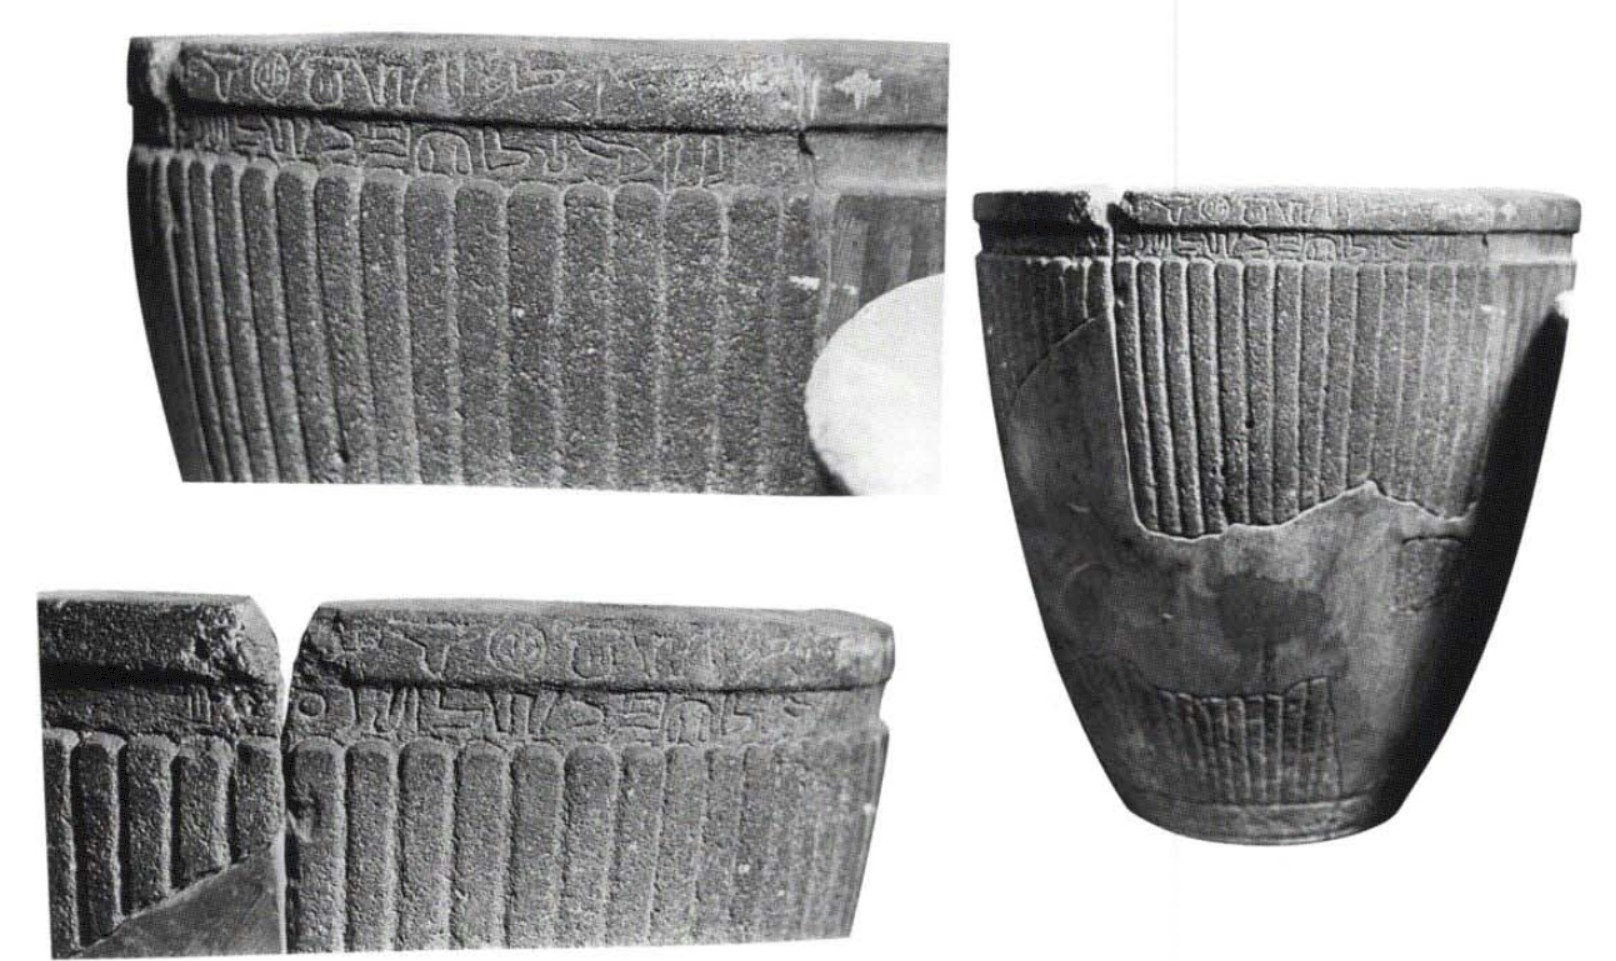
\includegraphics[width=\textwidth]{../../Mídia/aleppo23.jpg}
	\end{center}
	\begin{center}
		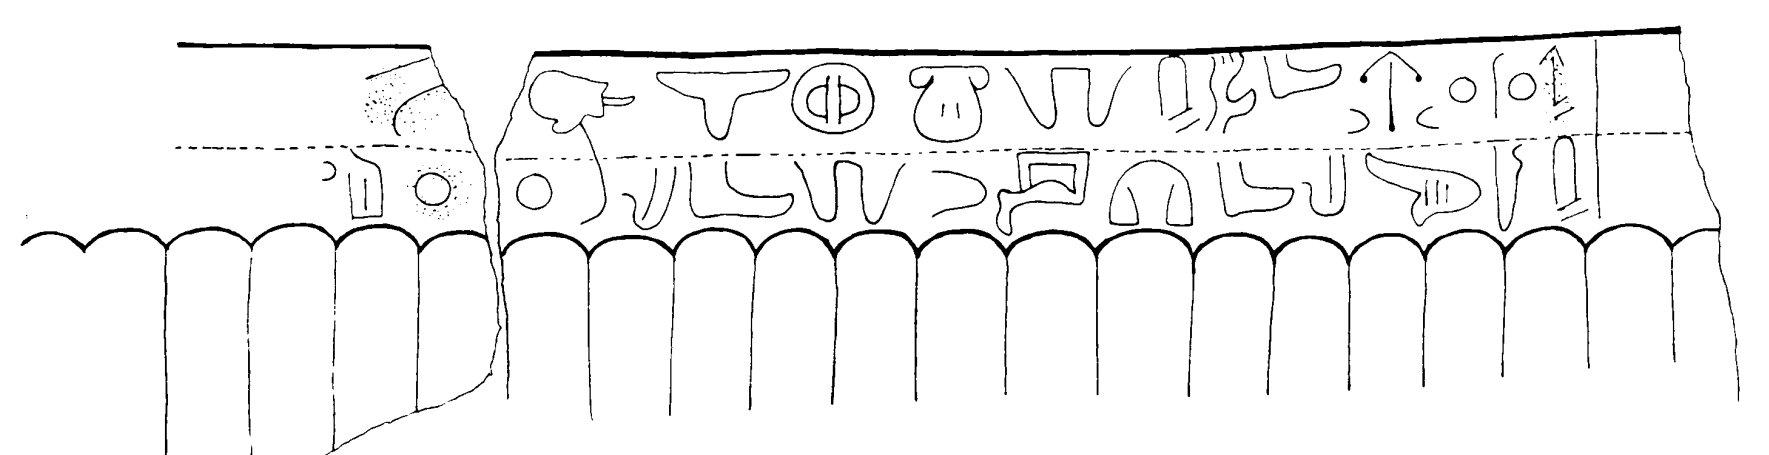
\includegraphics[width=\textwidth]{../../Mídia/babylon3.png}
	\end{center}
	\caption{Babylon 3. Diâmetro: 0.66m.; Profundidade (interna): 0.67m. Imagens
		produzidas e traçado feito por \textcite[\emph{plate} 212]{CHLI_1_3}.
		Atualmente no \foreignlanguage{german}{Vorderasiatisches Museum}, Berlin, no. VA Bab. 1507.}\label{fig:babylon3}
\end{figure}

\ex.\ag.{\Large 𔖪𔓱𔗬𔗷} {\Large 𔗎𔔯𔗏𔗧𔑣𔐤} {\Large 𔑵𔑣𔓱𔗔} {\Large 𔓢𔑞𔕸𔗐} {\Large 𔖖𔓢𔕙𔑣}
{\Large 𔐎𔐤} {\Large [𔑇]𔗬𔑯}\\
za-ia-wa/i-a\hspace{10pt} ``SCALPRUM''-ka-ti-na\hspace{10pt}
CERVUS\textsubscript{2}-ti-ia-sa\hspace{10pt} TONITRUS.HALPA-pa-ni\hspace{10pt}
DEUS.TONITRUS-hu-ti\hspace{10pt} PRAE-na\hspace{10pt} [PONERE]-wa/i-ta\\
zaya=wa katin(a) Runtiyas halpawani Tarhu(n)ti paran tuwa-ta
\bg. zaya=wa katin(a) Runtiyas halpawani Tarhu(n)ti paran tuwata\\
\Det{}\Acu{} vasilha.\Neut{}\Acu{} R.\Com{}\Nom{} halabeu.\Dat{} T.\Dat{} \Prep{} colocar-3\Sg\\
Esta vaso Runtiyas colocou em frente (=dedicou) ao Tarhunta halabeu.

